\section{Presentation Logic Layer}

%What pages will be present in your project? briefly indicate how your web site will be organized

The following pages are an example of the pages available:

\begin{itemize}

\item \textbf {Home Page:} This serves as the landing page for the website. It showcases top-rated movies and provides a link to the login page for users. The page features a menu bar accessible across the site post-login, offering options such as Movies/TV shows, Celebrities, and Awards and Events. Additionally, it includes a search bar allowing users to specify their search by title, episode, celebrities or companies.
\item \textbf {Movie Page:} This page displays all the information about the movie, including the title, actors/actresses, director, reviews, rating and the link where we can watch the trailer of the movie.
\item \textbf {Login Page:} Users are required to enter their email address, name, surname and password to access the web application's features and content.
\item \textbf {Person Page:} This section allows users to access information about actors/actresses, directors, writers and the movies they are associated with. Users can view details such as filmography, awards won, and biography.
\item \textbf {Add/Delete Movies (Admin Page):} This page allows the admin to add or delete movies to the database.
\item \textbf {Add Persons (Admin Page):} This page allows the admin to add persons (actors/actresses, directors, writers) to the database. Admin can create person form such as name, surname, bio, role, birth place, birth date, photo link.
\item \textbf {Watchlists (User Page):} This feature enables users to curate a list of movies they intend to watch later. It serves as a convenient reminder for users to keep track of movies of interest.
\item \textbf {Your Ratings (User Page):} Users can view statistics related to movie ratings, such as the average rating of movies viewed by the user. 
 \item \textbf {User Profile (User Page):} This page allows users to view and modify their personal information stored on the platform. Users can update details such as their first name, last name, username, email address and password.
  \item \textbf {Your Lists (User Page):} The user of the application can add movies to his lists of movies, create a new list or delete them.
 
\end{itemize}

\subsection{Home Page}

The home page is the main page of our website. In this page, we have some movie suggestions for 2 categories; best of all and top picks for this week. We choose best of all movies based on overall ratings and display the first 6 of them in our home page. For top picks, admins choose randomly (or last week's most watched first 6 movies) and they are also displayed in home page. 

\begin{center}
   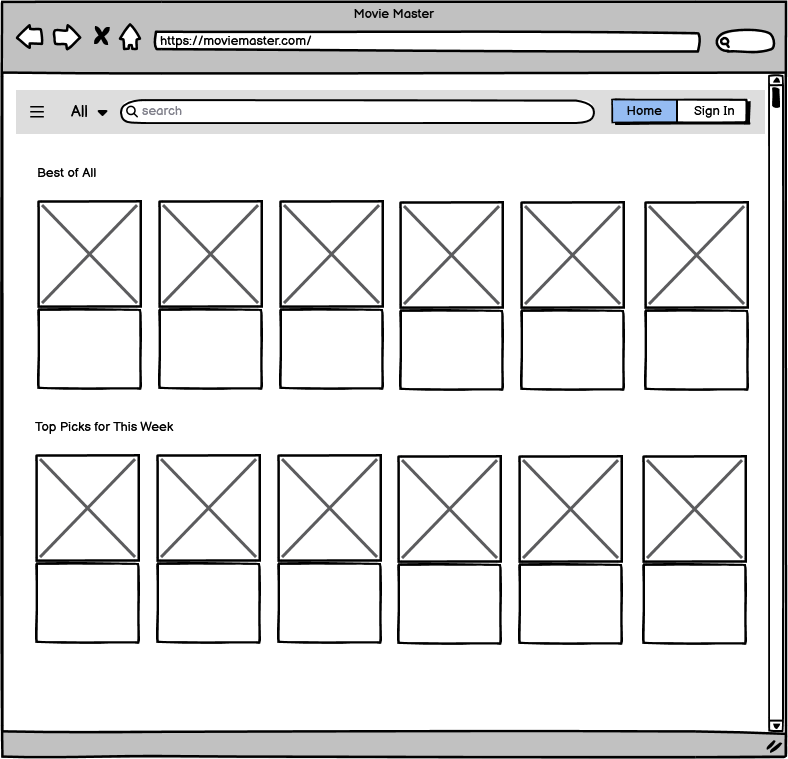
\includegraphics[width=12cm, height=9cm]{pictures/Home Page.png}
\end{center}

Home page contains a search bar to search movies/tv shows/celebrities directly. They can search from all of our content or they can narrow down the search area by selecting the specific category. They can select the category via submenu leftside of the search bar. 

\begin{center}
    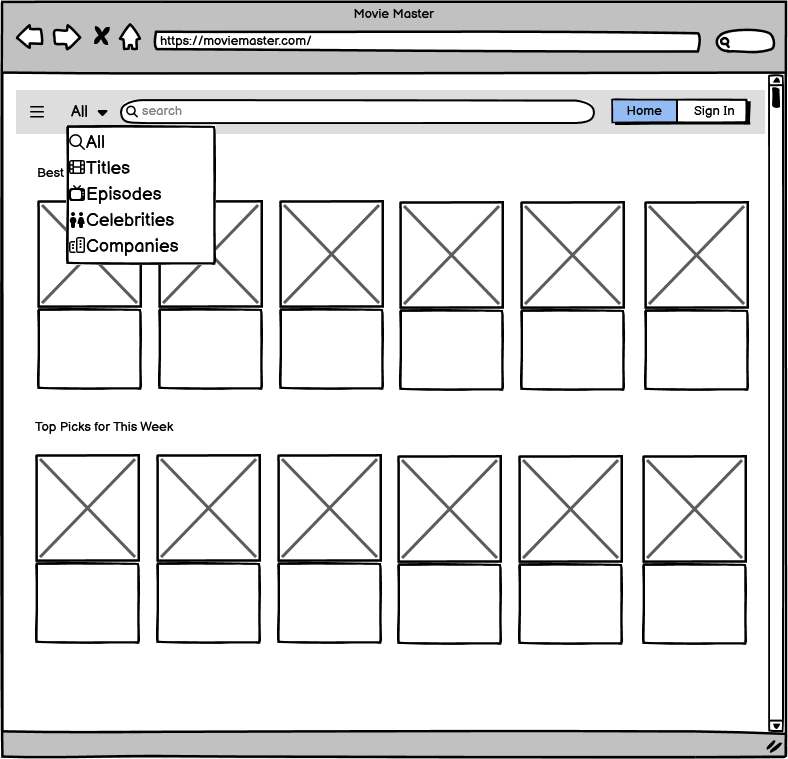
\includegraphics[width=12cm, height=9cm]{pictures/Search Bar Menu.png}
\end{center}

\newpage
Also, if the user wants to go to the related main page (movies, tv shows, celebrities, etc.), they simply can click the 3-line submenu button and select the category they want. 

\begin{center}
    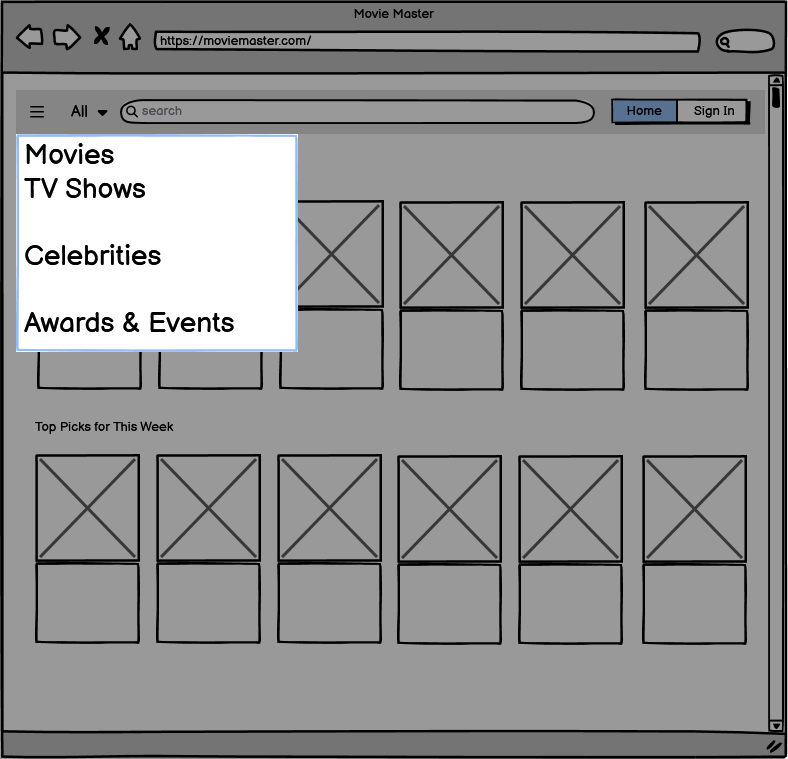
\includegraphics[width=12cm, height=9cm]{pictures/Main Menu.png}
\end{center}

We also have 2 other buttons on the Home page. One of them is Home button and the other is Sign In button. Sign In button directs user to Login/Sign Up pages, and user can choose which one is suitable for him/her. Home page directs users to home page regardless of which page they are. 

\subsection{Login/Signup Page}

%For the main pages put a mockup and describe it in detail.
\begin{center}
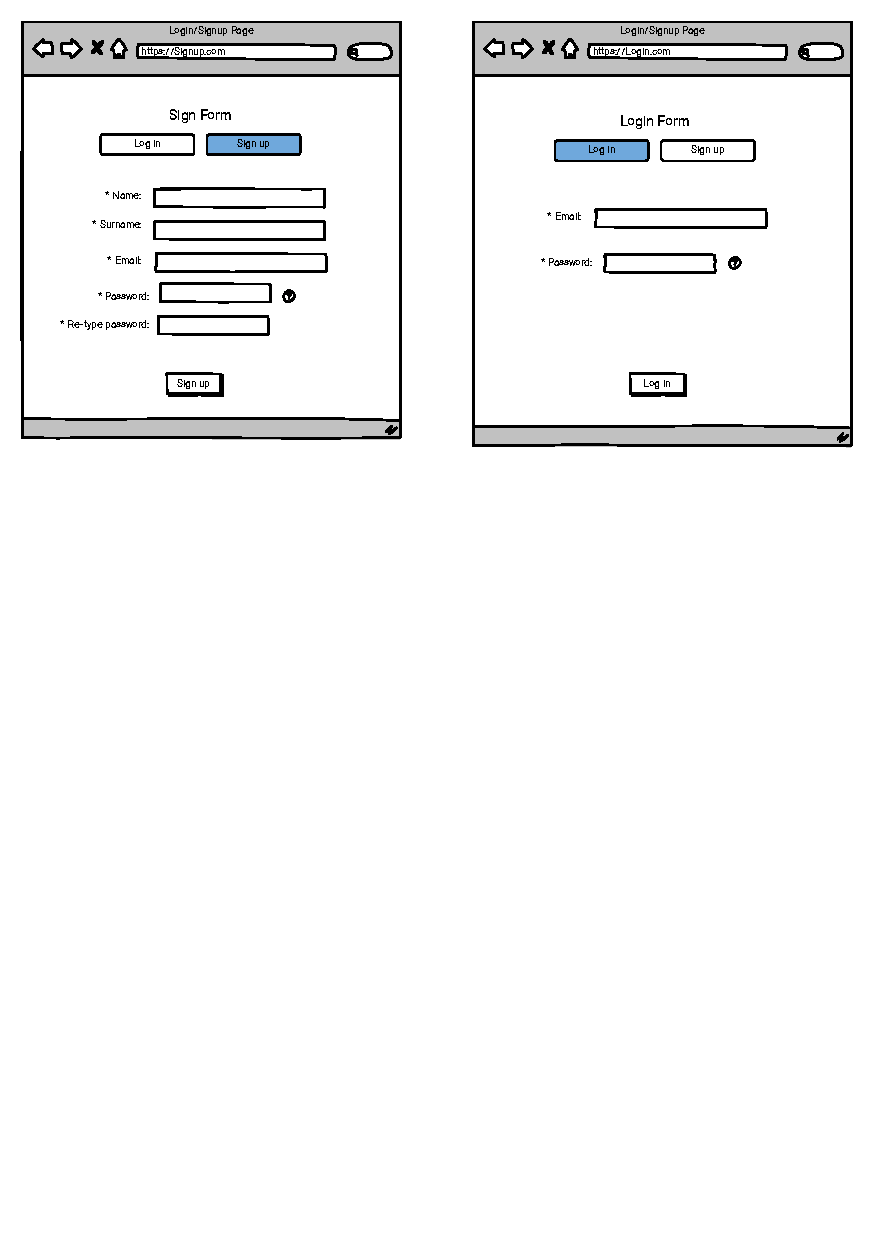
\includegraphics[width=17cm, height=7cm]{pictures/Login Signup Form.pdf}
\end{center}

The login page is the gateway to authenticate users by requiring them to input their credentials —an email address and a password— before granting access to the platform's features and content. The form consists of two boxes, one to gather the username and the other for the password.
The signup page serves as the entry point for users who wish to create a new account on a website. Its primary function is to collect essential information from users.These input fields include fields for the user's email address,name, surname, password and re-type password. 

\subsection{User Page}

%For the main pages put a mockup and describe it in detail.
\begin{center}
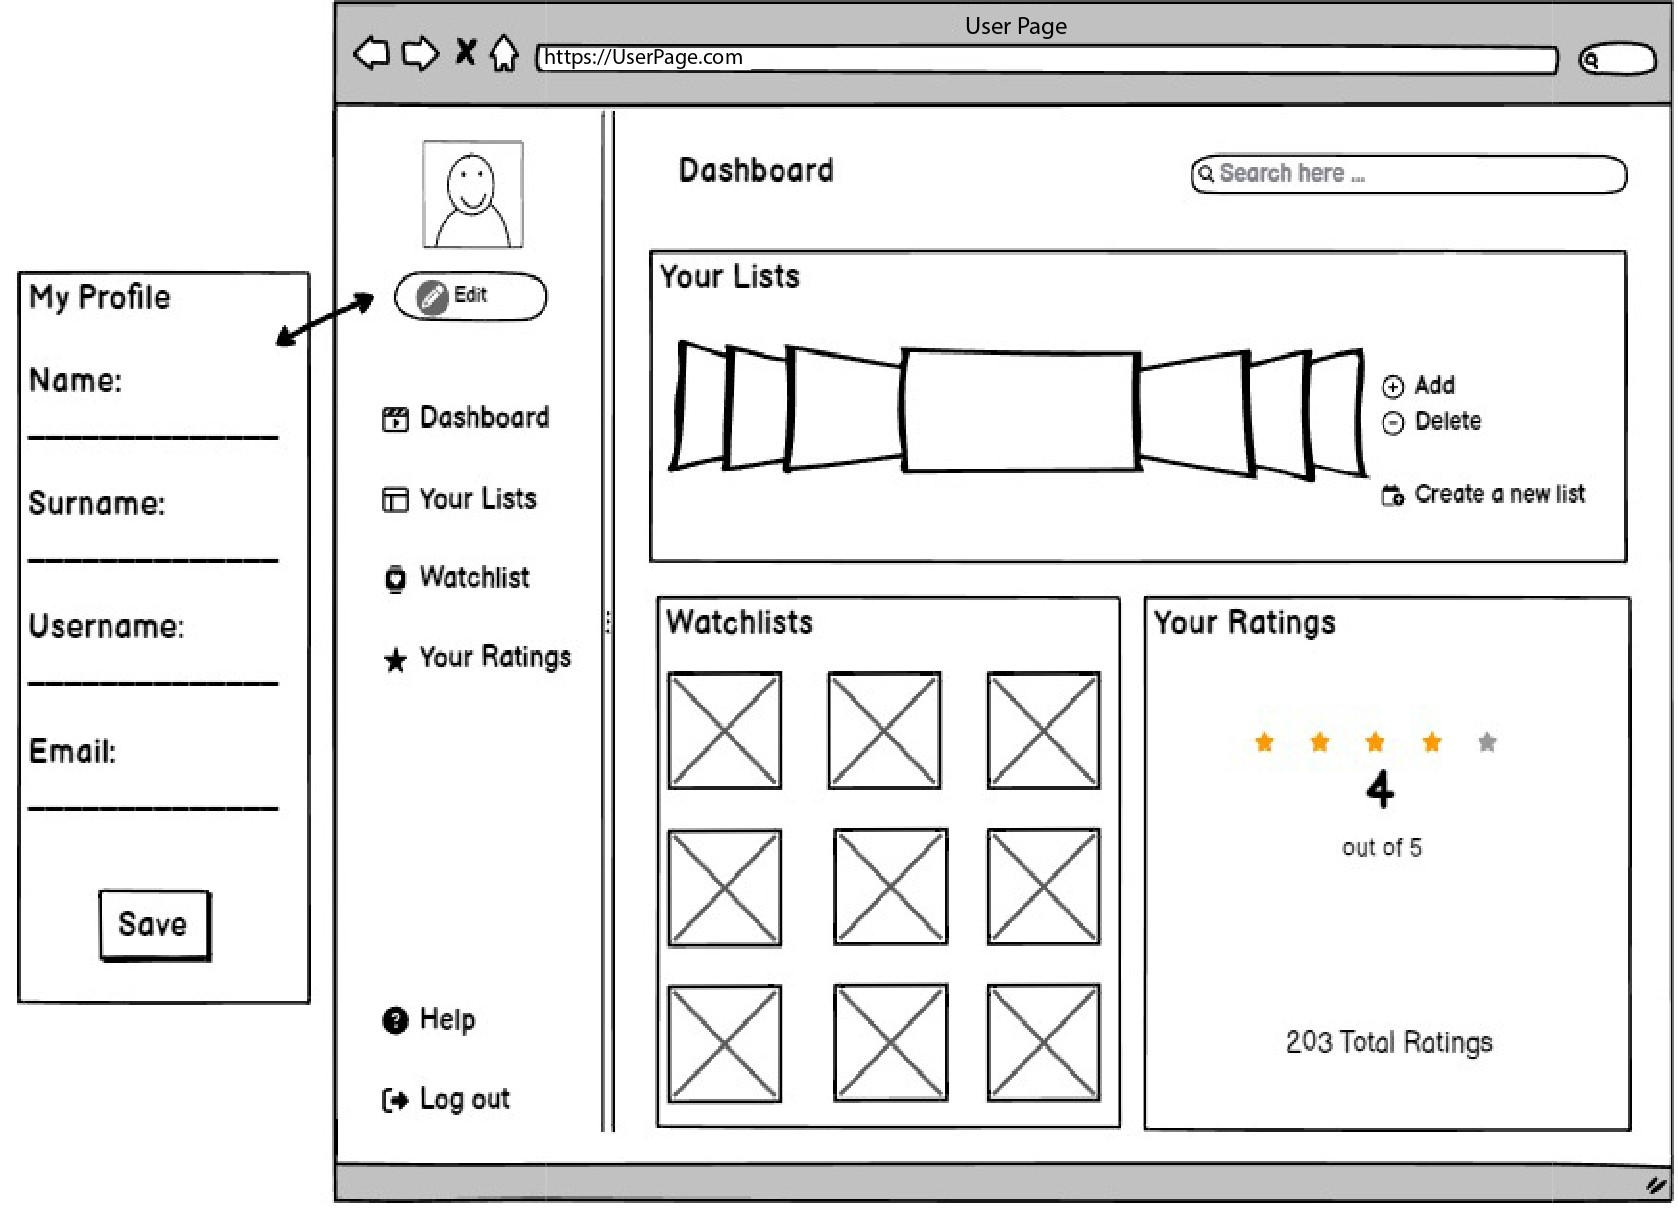
\includegraphics[width=12cm, height=9cm]{pictures/UserPage.jpg}
\end{center}

This page empowers users with various functionalities: 
\begin{itemize}
\item  Movie Management: Users can effortlessly add or remove movies from their lists. This feature extends to all users, enabling them to curate a personalized selection of movies they plan to watch in the future. It serves as a handy tool for users to maintain a catalog of movies they find intriguing.
\item  Rating Statistics: Users gain access to insightful statistics concerning movie ratings. This includes valuable data such as the average rating of movies viewed by the user, offering a comprehensive overview of user preferences and popular content.
\item  User Profile Editing: Users are provided  to review and modify their personal details stored on the platform. This encompasses essential information like first name, last name, username, email address, and password. 
\item  Watchlist: Users can maintain a 'Watchlist' within the application, where they compile movies they intend to watch in the future. This feature allows users to easily track and manage their cinematic interests, add new titles, remove ones they lose interest in, and organize the list based on preference. 
\end{itemize}

\subsection{Admin Page}

%For the main pages put a mockup and describe it in detail.
\begin{center}
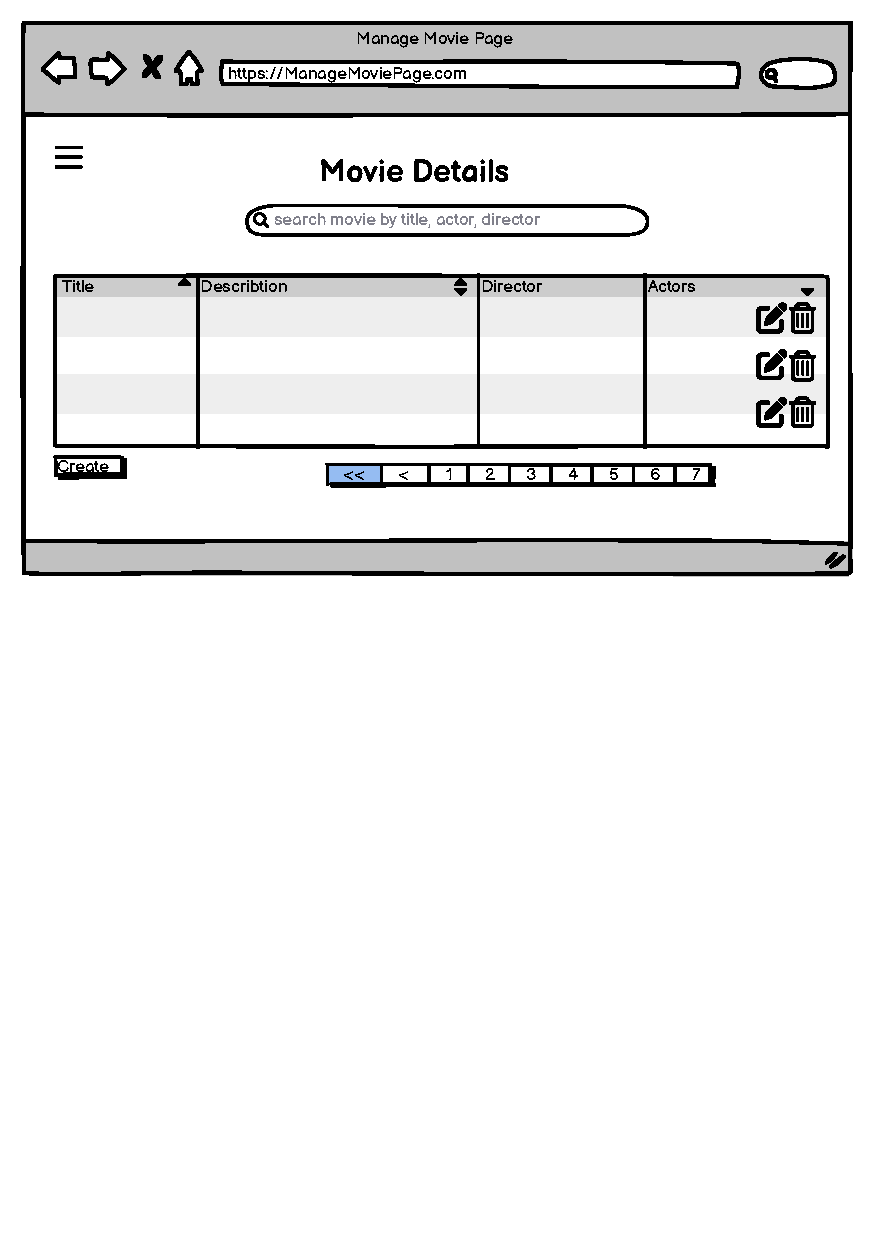
\includegraphics[width=12cm, height=9cm]{pictures/AdminPage.pdf}
\end{center}
Add/Delete Movies: This dedicated section empowers administrators to seamlessly manage the application's movie database. Administrators have the capability to add newly released movies or remove outdated entries from the database. The administrator adds the title,director, genre, release data, trailer URL.

Add/Delete Persons: Within this essential feature, administrators can maintain a comprehensive database of individuals involved in the film industry, including actors, actresses, directors, and writers. Administrators are equipped with a user-friendly form interface to facilitate the addition of new persons to the database. The form typically includes fields such as name, surname, biography, role (e.g., actor, director), birthplace, birthdate, and a link to their photo. 

\subsection{Movie Page}

%For the main pages put a mockup and describe it in detail.
\begin{center}
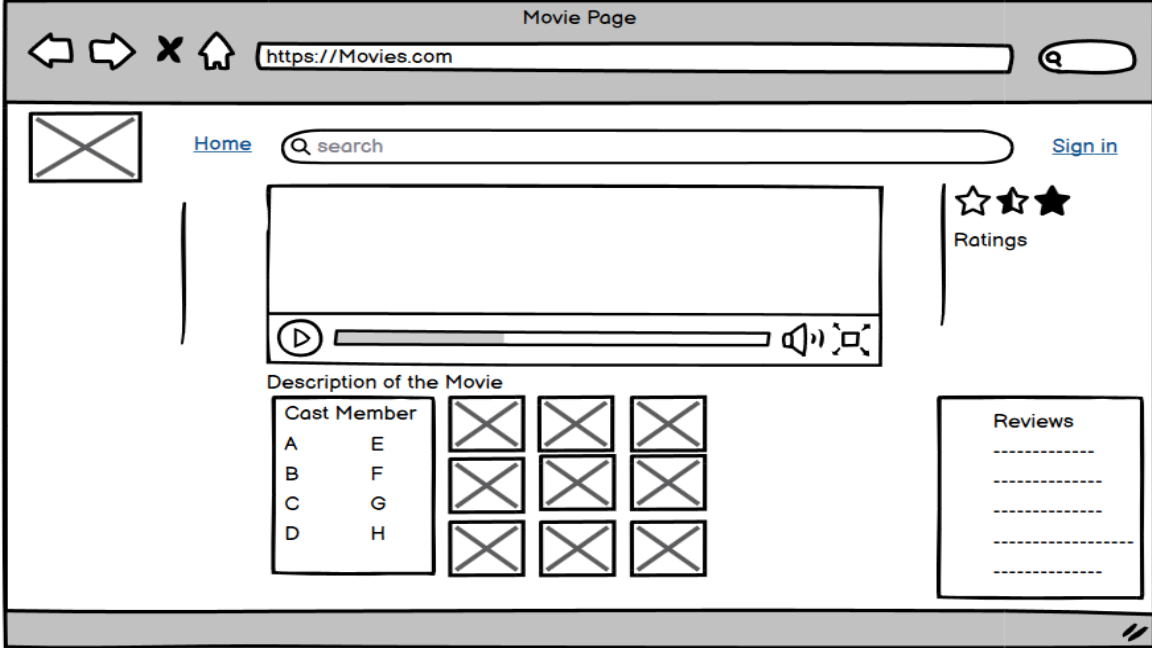
\includegraphics[width=12cm, height=7cm]{pictures/Movie Page.png}
\end{center}

The book page  shows everything you need to know about a movie, like its title, cast member, storyline. Central to the book page's functionality is its interactive nature, which empowers users to actively engage with the movie's content. Users have the opportunity to leave their mark on the narrative by sharing their insights through personalized evaluations and reviews. Through a user-friendly rating system, individuals can express their appreciation or critique of the movie.


\subsection{Persons Page}

%For the main pages put a mockup and describe it in detail.
\begin{center}
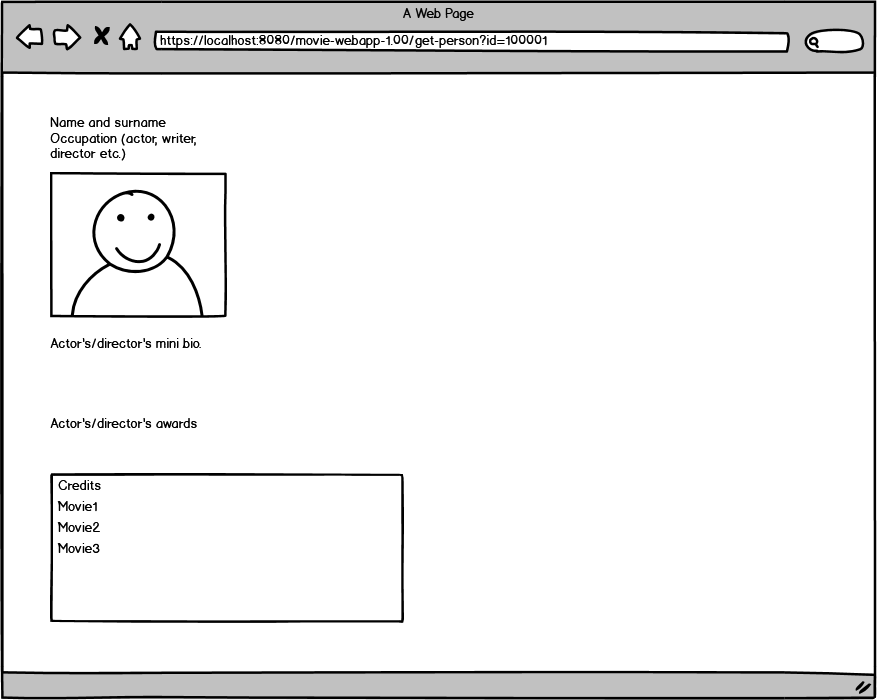
\includegraphics[width=12cm, height=10cm]{pictures/Person_prototype.png}
\end{center}

This page displays data about a person by their id. It contains:
\begin{itemize}
\item Name and Surname: Name and Surname of the person.
\item  Occupation: Role of the person (director, writer, etc.)
\item  Photo: photo of the person.
\item  Short bio: small biography of the person.
\item  Awards: awards of the person.
\item  Credits: movies in which the person was involved.
\end{itemize}

\subsection{Add Person Page}

%For the main pages put a mockup and describe it in detail.

\begin{center}
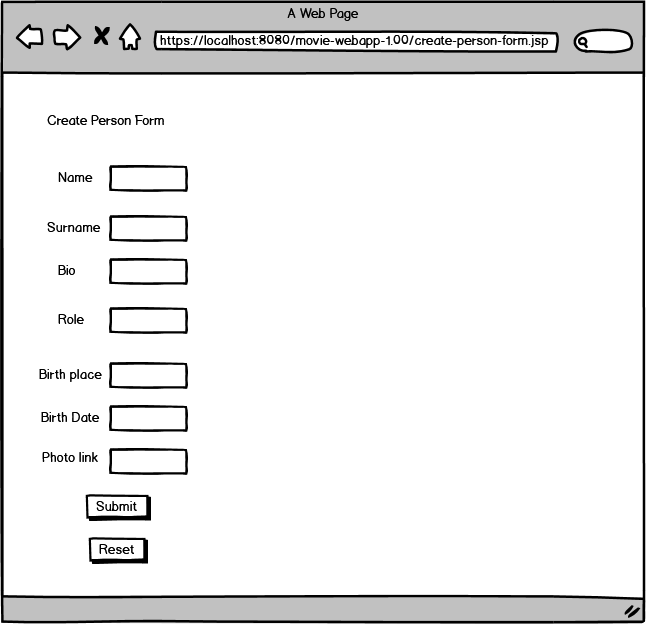
\includegraphics[width=12cm, height=10cm]{pictures/Create Person Form.png}
\end{center}


This page displays form that user needs to fill to add a person to the database. It contains:
\begin{itemize}
\item Name field: Name of the person.
\item Surname field: Surname of the person.
\item  Short bio: Small biography of the person.
\item  Role: Role of the person (director, writer, etc.)
\item  Photo link: Link to the photo of the person.
\item  Birth place: Place of birth of the person.
\item  Birth date: Date of birth of the person.
\end{itemize}

\subsection{Add Movie Page}

%For the main pages put a mockup and describe it in detail.
\begin{center}
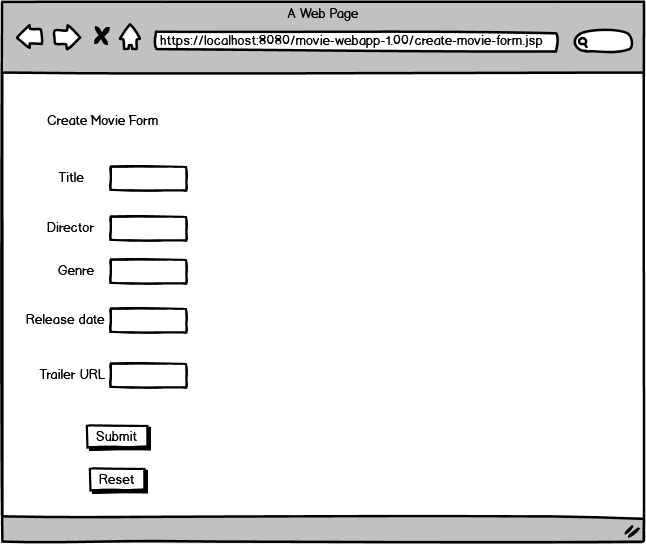
\includegraphics[width=12cm, height=10cm]{pictures/Create Movie Form.png}
\end{center}

This page displays form that user needs to fill to add a person to the database. It contains:
\begin{itemize}
\item Title: Title of the movie.
\item Director : Director of the movie.
\item  Genre: Genre of the movie.
\item  Release date: Release date of the movie.
\item  Trailer URL: Link to the trailer of the movie.
\end{itemize}
